\documentclass[10pt]{report}
\usepackage{graphicx}
 \setlength{\parskip}{6.0mm}
 \setlength{\parindent}{0pt}
 \begin{document}
 Villigen \& Beijing \today \\
 
 Respected Referee
 
 we have carefully answered all you question and implemented many
 of your suggestions. Our response is clearly stated, below each of your raised points.
 
 With the best regards

Andreas Adelmann \& Jianjun Yang

Point 1. It contains computer-insider jargon. For example, algorithm 2 still contains
$i_{NB}=i_{NB}+1$. I understand this means ``replace the value in the memory
location labelled $i_{NB}$ with its value when incremented by 1''.
Nevertheless, it is mathematical nonsense.

 \vspace{+2mm}
 {\it {\bf Our response}  We removed the so called computer-insider jargon with:} \\ increment$(i_{NB})$, and
 hopefully it is now clear that simply the count of neighboring bunches is incremented by one.
 \vspace{+2mm}
 
Point 2. Quantitative comparison with PICN\\  
{\it {\bf Our response}} We contacted the author of PICN code, S. Adam, 
and quantitatively compared the rms size after each turn on both the longitudinal and radial directions, the result are shown in the following figure.
And we discuss the reason of the difference with S. Adam in detail.
Accordingly, in the paper we more carefully justified our reasoning in comparing PICN and OPAL-CYCL and the conclusions are rephrased. 

  \begin{figure}[H]
    {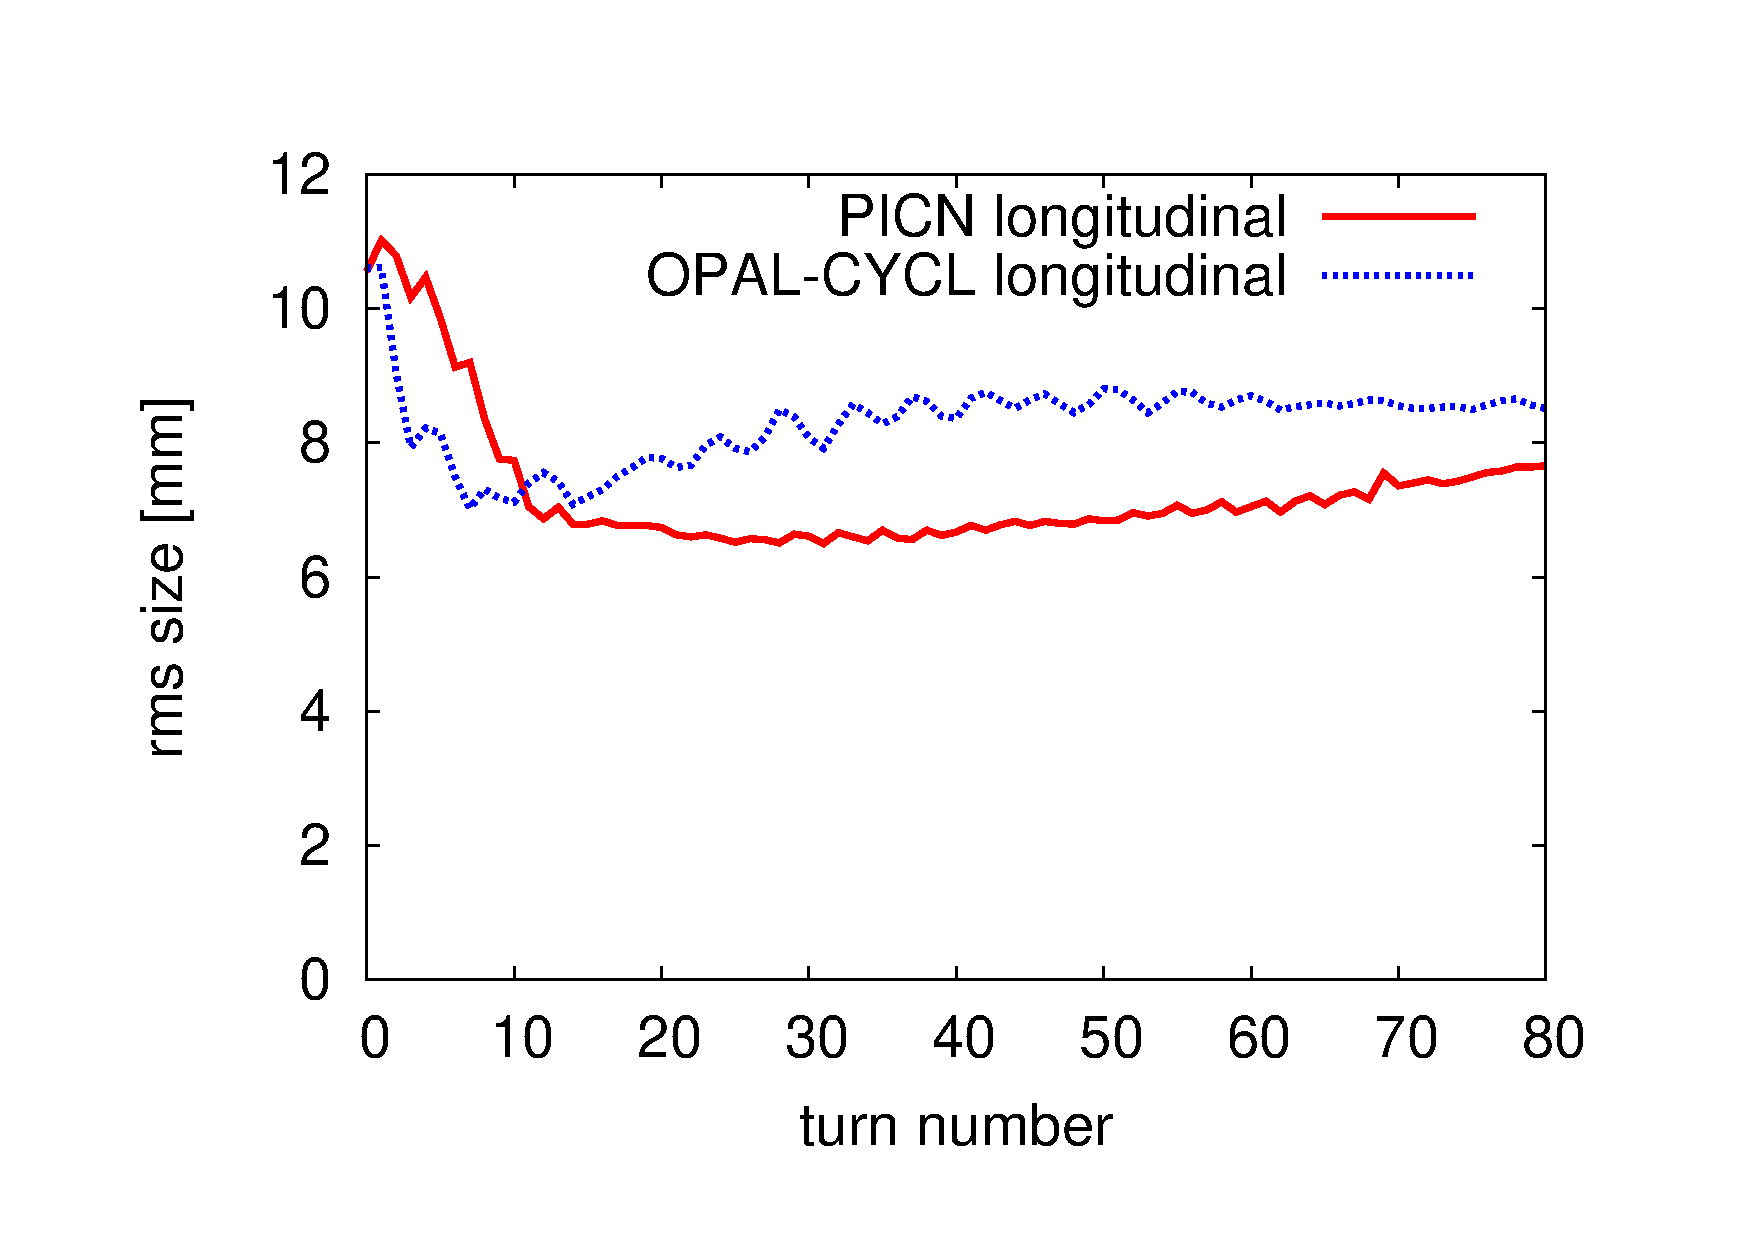
\includegraphics[width=14cm]{compare-long.pdf}}
    {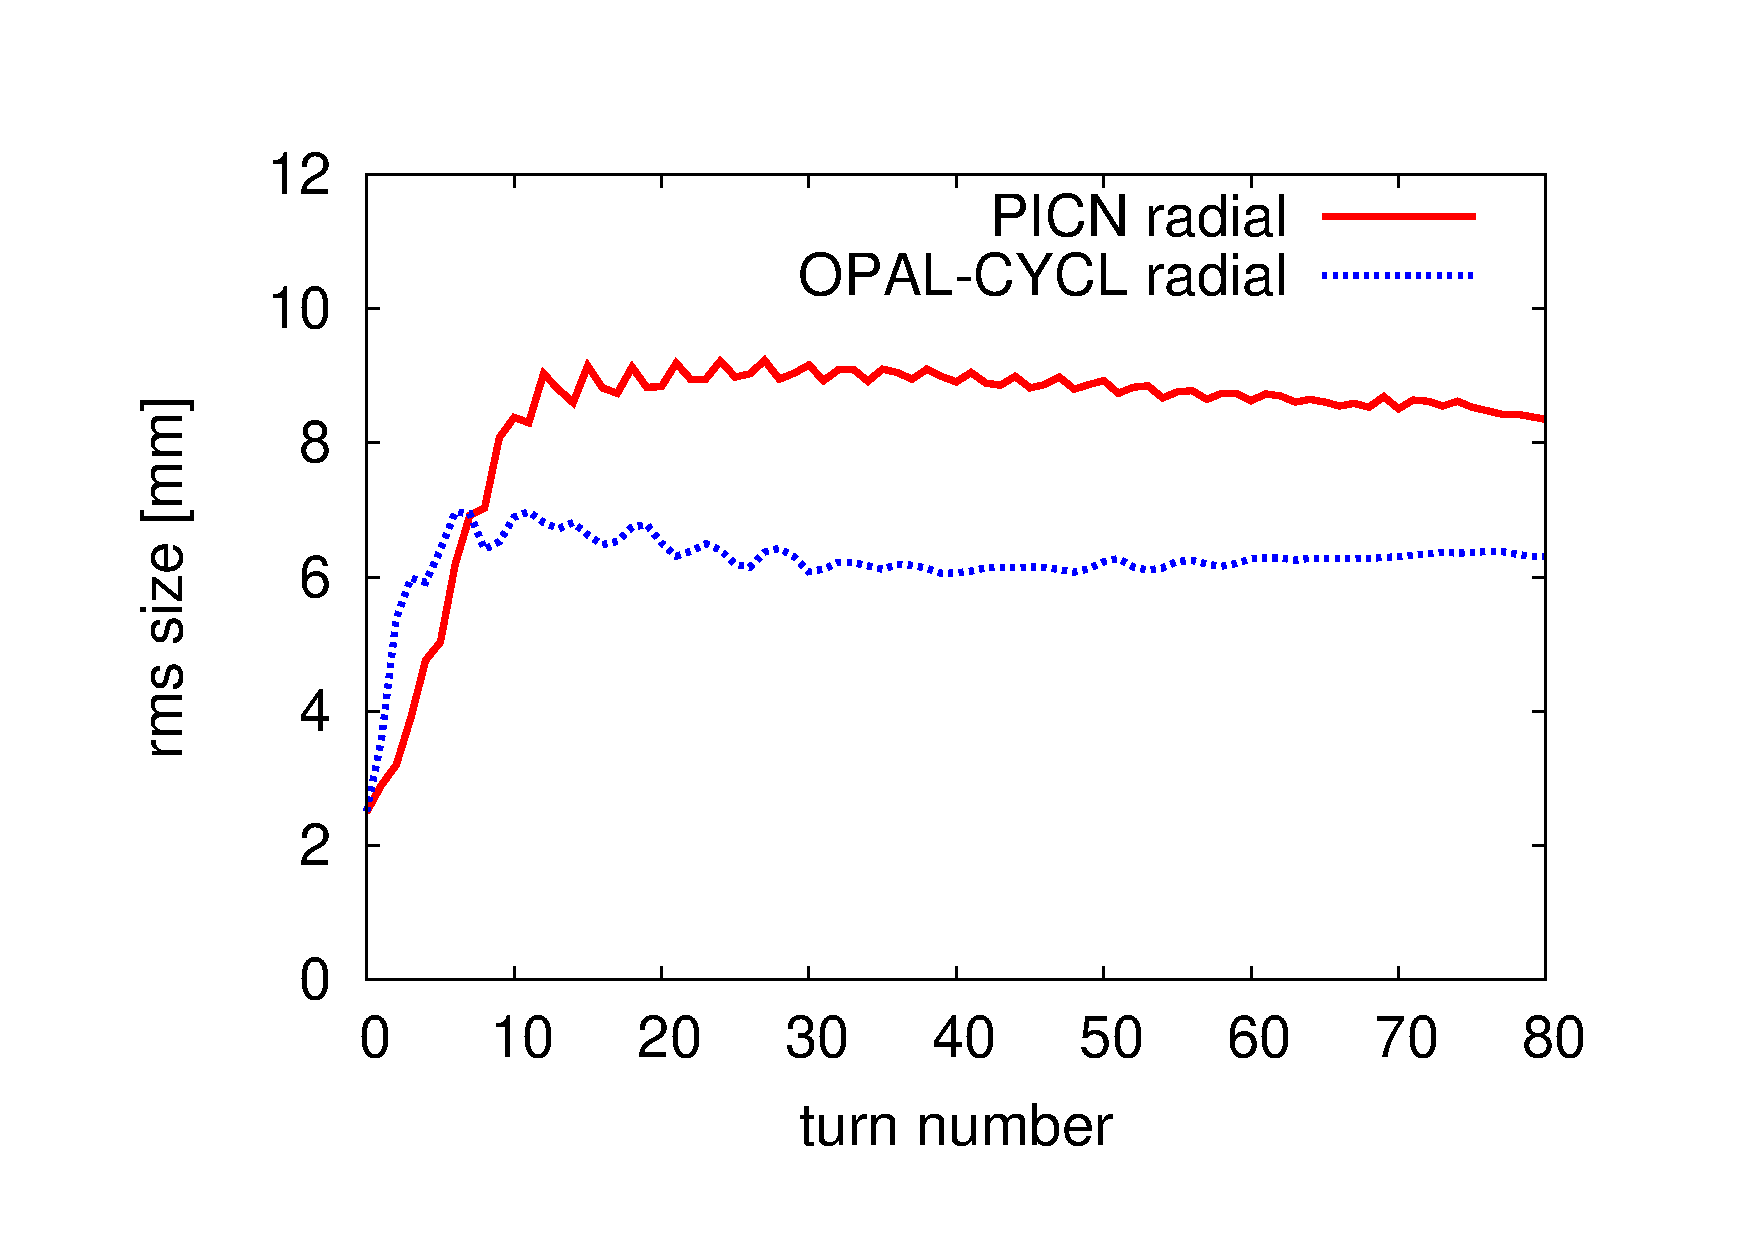
\includegraphics[width=14cm]{compare-rad.pdf}}
    \caption{comparison of the rms size by PICN and OPAL-CYCL}
    \label{fig1}
  \end{figure}

To the second issue of Point 2 raised by the referee: \\
{\it {\bf Our response}}  As Gordon explained in [10] the particle motion in a cyclotron is always perpendicular to the force
resulting in a vortex motion. In order to obtain the observed sharpening of the distribution we
need an additional, azimuthal force. A possible explanation of the origin of this force is due to the observed broken spherical symmetry when considering neighboring bunches in the simulation. However more  efforts are needed in order to understand this effect in greater detail.

[10] M. M. Gordon, in Proc. 5th Int. Conf. on Cyclotrons and their Applications (Oxford, 1969), p 305


 \end{document}
